\section{Biology Primer}\label{sec:Biology}

This section will start with an introduction to the natural aspect of biology, including what DNA is and how it can be analysed.
Genomic biology is a wide topic, hence this thesis will stick to what is relevant for it.
Later, this will be linked to how researchers can use sequencing technologies in order to make new inferences.

First is a description of what Deoxyribonucleic Acid (DNA) is.
Each organism is made up of cells, and each cell has different components, but in the center is a nucleus which is the driver of everything else, and within this nucleus is the DNA~\cite{CellBiology}.\@
The actual biology is more complicated than this, however, this is as far as the reader needs to understand about the cell structure.

The DNA contains a sequence of bases: Adenine, Cytosine, Thymine, and Guanine.
For the representation in this thesis, each base is represented by a single character: $ACGT$, corresponding to the first letter of the name of each base.
Each base has a pair, where the bases $A$ and $T$ bind together, and $C$ and $G$ also bind together.
These base pairs then attach to a sugar phosphate backbone to form the double helix of the DNA~\cite{DNA}.
Figure~\ref{fig:DoubleHelix} shows the different parts of the double helix visually.
Note that this representation is usually represented as a twisted ladder, but for clarity, a straightened ladder was chosen for the visualisation.

\begin{figure}[t]
  \centering
  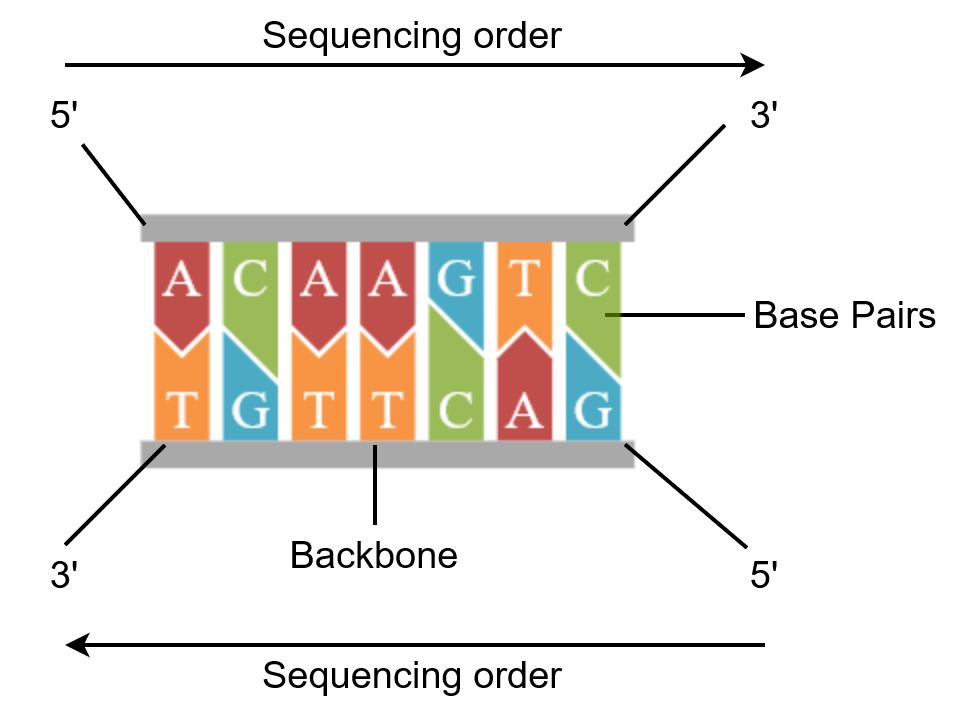
\includegraphics[width=0.55\textwidth]{images/DoubleHelix.png}
  \caption{The double helix of the DNA showing the 2 backbones and the attached base pairs. The visualisation was created using \url{https://www.petercollingridge.co.uk/tools/draw-dna/}}\label{fig:DoubleHelix}
\end{figure}

It is unfortunately very difficult to sequence an entire DNA strand at one go with current technologies.
Instead, a DNA of a sample is cloned multiple times, fractured, and read fragment by fragment~\cite{ShotgunSequencing}.
A sample may have multiple cells from different species, thus having multiple different DNA genomes jumbled together.
Sequencing can either be done using shotgun sequencing~\cite{ShotgunSequencingOriginal}, where each part of the DNA strand has an equal chance of appearing in the dataset, or targeted sequencing~\cite{TargetedSequencing}, where only certain parts of the DNA strand are targeted.
A single fragment is called a read.
The two types of this sequencing are short read sequencing (SRS) and long read sequencing (LRS)~\cite{SrsVsLrs}.
Longer reads are of course preferable because researchers can see more of a genome at a time, whereas with shorter reads, constructing a genome, which is discussed in Section~\ref{sec:DBG}, takes much longer due to the need for assembling many more reads together.
A genome is the full DNA string of a cell of an organism.
However, SRS is currently much more accurate than LRS~\cite{LrsChallenges}.
Accuracy in this case means that the sequenced bases are correct, and an error might be a base-flip, where, for example, an $A$ may be sequenced as a $C$.
Other sources of errors may be missing bases or the addition of non-existent bases.
Cost is also a big factor.
Two big players in these fields are Oxford Nanopore\footnote{\url{https://nanoporetech.com/}}, which perform LRS, and Illumina\footnote{\url{https://www.illumina.com/}}, which perform SRS and were the first to drop the cost of sequencing the full human genome to under \$1000~\cite{LrsChallenges}.
Illumina have been around for almost 20 years now, and have taken a large market share since lots of algorithmic pipelines are based on their technology~\cite{SrsVsLrs}.

To read the DNA, a messenger RNA (mRNA) is used~\cite{mrna} in a method called transcription.
This reads a single strand of the DNA and, luckily, nature has evolved such that the strands are always read from the 5' (five prime) end to the 3' end, as visualised in Figure~\ref{fig:DoubleHelix}.
This means that researchers have more information on the direction of the read, though one still can not know from which of the two strands the read comes from.
A technique that is often used is to also consider the reverse complement of a read.
The reverse complement of a read is the whole string reversed and the bases replaced by their pairs~\cite{ReverseComplements}.
From Figure~\ref{fig:DoubleHelix}, the first strand of the read may be \textit{ACAAGTC}, whereas the reverse complement is \textit{GACTTGT}.\@
Note that both strings may be sequenced with equal probability and it is not possible to know from which strand each string originates from just by looking at the two of them.
One would need to assemble them with other reads in order to know where they belong.

De novo assembly is when different reads are combined together using overlaps in their prefixes and suffixes to construct the full reference genome~\cite{DeNovoAssembly}.
The na\"ive algorithm for this process is to try out all combinations of read pairs and positions and see where they fit best within the context of the whole genome, without knowing what the genome actually looks like~\cite{EulerianPath}.

Ideally, every cell in a body would have the same DNA sequence.
However, mutations do exist, and mutations also develop over time and inevitably lead to aging.
However, many mutations across different parts of the body may lead to severe diseases~\cite{Mutations}.
Hence, analysing these mutations within a genome is one use case for how researchers can use such DNA data and alignment techniques in order to find out more about, for example, the condition of a patient.

To analyse these mutations, alignment can then be used, after a reference genome has been constructed, where the reads of a new specimen are aligned to this genome.
Alignment means to find the best position within the reference genome where there are the least differences between the sequences~\cite{Alignment}.
Gaps may also occur when certain types of mutations occur, and they may also manifest themselves as a character flip within the DNA string.
One use case of alignment could be to find these mutations in the genetic code between healthy people and those with a certain disease, such as forms of cancer~\cite{BreastCancer}.
Figure~\ref{fig:Alignment} shows an example of two aligned reads with some differences.

\begin{figure}[t]
  \centering
  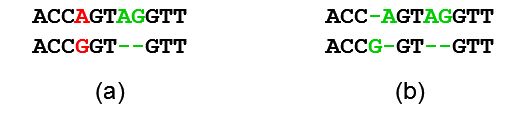
\includegraphics[width=0.55\textwidth]{images/Alignment.png}
  \caption{Two reads aligned to one another. Note that (a) and (b) represent the same two reads, but in one representation the first difference is represented  as a character flip, in red. Meanwhile, in (b) it is represented as 2 separate insertion and deletions in green. Gaps are represented with the '-' character. Since the reference genome is not known in this case, the second difference may be either an insertion or a deletion, or a mixture of both. When doing assembly, these sequences would instead be correlated with more reads to check their correctness and increase the confidence in the accuracy, rather than being compared to the reference genome. If this is all the information that was available, option (a) would be the preferred option to choose as there are fewer operations to align the two sequences.}\label{fig:Alignment}
\end{figure}

Contigs are also explained as they will be a useful concept in Section~\ref{sec:DBG}, mostly unitigs are discussed.
A contig forms when a set of reads is assembled together.
The assembled sequence from end to end is called a contig.
The term \textit{contig} comes from the word \textit{contiguous}, as the reads in the contig set are contiguous~\cite{Contig}.
This contig might contain some uncertainties, due to the mutations described previously.
Figure~\ref{fig:AssemblyAndAlignment} shows a more complex example of alignment with contigs.

\begin{figure}[t]
  \centering
  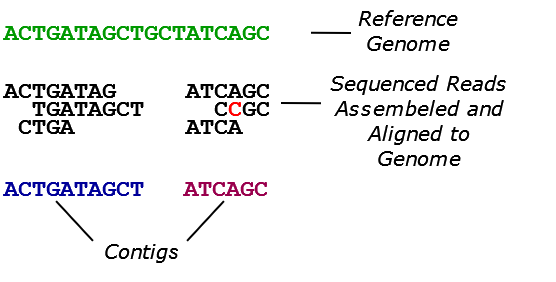
\includegraphics[width=0.55\textwidth]{images/AssemblyAndAlignment.png}
  \caption{A more complex diagram of alignment and assembly. The reference genome is given in green at the top, with the newly sequenced reads, assembled and aligned to the reference genome, in the middle, and the contigs extracted from those reads at the bottom. Note that if the reference genome was not known, then this would be doing De novo assembly, rather than alignment, to try to construct the genome without knowing it.}\label{fig:AssemblyAndAlignment}
\end{figure}

The data is stored in what are known as FASTA and FASTQ files.
An example of the FASTA format may be seen in Figure~\ref{fig:FASTA}.
This format consists of multiple sequences, each starting with the '>' character, followed by the title of the sequence, which is then followed by the sequence itself on the next line.
This sequence can be on multiple lines~\cite{FastaAndFastq}.
Besides the ACGT characters, which are sometimes in uppercase and other times in lowercase, the character N is sometimes used to signal an ambiguous base\footnote{\url{https://knowledge.illumina.com/software/general/software-general-reference_material-list/000003560}}.
The sequences may be genomes or reads.

The second file format is FASTQ, which contains additional information about the quality of each base in the read~\cite{FastaAndFastq}.
An example can be found in Figure~\ref{fig:FASTQ}.
This format starts with the '@' character followed by the title, and the read on the next line which can be of multiple lines similar to the FASTA format.
Then a '+' is added on the next line, which may or may not be followed by the same title of the sequence on the same line, and lastly the quality string on the next line (or lines) which should be of equal length as the sequence.
The characters of the quality string indicate the confidence in the corresponding base at that same index within the sequence.
The specifics of how these characters are interpreted will not be delved into, as they are not relevant to the rest of the text.

FASTA files are usually used for representing reference genomes, while FASTQ files are used for raw read data since they can also contain the quality string.
Unfortunately there is not a single standard for the file formats, although there are some attempts at creating some\footnote{\url{https://www.ncbi.nlm.nih.gov/genbank/fastaformat/}}.
Even the titles themselves can be of any form, as can be seen in the two examples.
The characters used for the quality string are also different between standards.
As such, writing a parser for these file formats can be a headache~\cite{FastaAndFastq}.
For this thesis, a scalable parser capable of supporting both FASTA and FASTQ files, or a mixture of both, was implemented, which is also capable of reading zipped and unzipped files.
This parser skips over title lines and quality strings, since these are not needed for this use case.

\begin{figure}
\centering
\begin{lstlisting}[basicstyle=\footnotesize\ttfamily]
>ERR345345.239 AJIJSDIO
ATCGTCACTAGCTAGCTAGCTACcagagctagtcagctagcactcagtcat
GCTCGAGTCAGC
>seq2
gtagcatcGATCGATCAGTGACNNNNNNNNNNNNNATGTCGAAAGAATAGTCGATG
CGATagtacgctcacgtacgactcgtc
>seq3
GAGTGAGTGCCCCtttaagagtattgtaGT
\end{lstlisting}
\caption{An example of a FASTA file with 3 sequences.}\label{fig:FASTA}
\end{figure}

\begin{figure}
\centering
\begin{lstlisting}[basicstyle=\footnotesize\ttfamily]
@ERR345345.239 AJIJSDIO
ATCGTCACTAGCTAGCTAGCTACcagagctagtcagctagcactcagtcat
GCTCGAGTCAGC
+ERR345345.239 AJIJSDIO
>)II8123))II328947289BA@@@@FFFFDFHFFHGHIGGGBFFAFGCF
;<B;@A5;5<DD
@seq2
gtagcatcGATCGATCAGTGACNNNNNNNNNNNNNATGTCGAAAGAATAGTCGATG
CGATagtacgctcacgtacgactcgtc
+
>)II8123))II328947289BA@@@@FFFFDFHFFHGHIGGGBFFAFGCF3))II
;<B;@A5;5<DD3))II3))II3))II
@seq3
GAGTGAGTGCCCCtttaagagtattgtaGT
+
@@@FFFFDFHFFHGHIGGGBFFAFGCF3))
\end{lstlisting}
\caption{An example of a FASTQ file with 3 sequences.}\label{fig:FASTQ}
\end{figure}

In the next sections, advancements in computer science algorithms will be discussed, which have made the analysis of such data more feasible and accurate.
